\subsection{Results from interviews}
There are several reasons why the current recruitment process needs to be optimized.
Firstly, a lot of time is spent communicating information back and forth between Accounting and Recruitment. 
Each department maintain their own data, in individual Excel spreadsheets, about the new employees. 
This should be optimized with the new HR-system.
Similarly time is spent communicating the information to the IT-department.
With a common system for keeping the information this could also be avoided, as IT could view the data within that system.

Secondly, the main reason for frustration in the IT-department is the short notice on some recruitments and the occasionally incomplete data.
The short notices are mainly rooted in recruitment of subcontractors in OMT.
While, the incomplete data occurs both with recruitments in Valcon and OMT.
Thirdly, time is spent on routine tasks, such as defining new initials, which could be automated if the data was kept in a standard format.

Part of the problem with incomplete data is that the initiators aren't all aware of which information the IT-department needs in order to set the new employee up correctly.

At Valcon, Accounting and IT support more standardized data, while Recruitment find it problematic because all data isn't necessarily available by the time of recruitment.
Furthermore, forcing standardized data might put additional pressure on the consultant/manager in charge of the recruitment, which should be avoided.
At OMT they also support more standardized data.

A visual representation of the problems at hand can be found in appendix \ref{app:ProblemChain}.
A transcript of the interviews can be found in appendix \ref{app:interviews}
\subsection{The numbers}
\begin{wrapfigure}{r}{0.5\textwidth}
\vspace{-20pt}
\centering
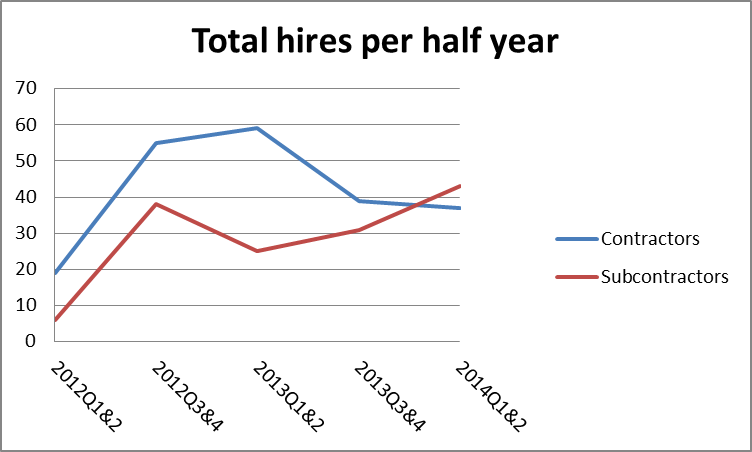
\includegraphics[width=0.45\textwidth]{appendix/total_hires_per_half_year.png}
\label{fig:total_hires_per_half_year}
%\caption{Total number of new hires per half year.}
\end{wrapfigure}
Looking at the number of new hires in Valcon we got an impression of the scope of the problem.
Even though there are some fluctuations there is a trend toward a growth in the number of hires.
This corresponds with the expressed business strategy of growth.
However, the data is not entirely conclusive, as we have only been able to look at the number of new hires within the last 30 months.
A table with all the numbers of new hires can be found in appendix \ref{app:recruitment_data} together with additional graphs.
\begin{comment}
\begin{enumerate}
	\item IT-department
	\begin{enumerate}
		\item Has an interest in automating as many processes as possible
		\item Current process forces them to put their other work aside to make time for the employment process
	\end{enumerate}
	\item Recruitment-department
	\begin{enumerate}
		\item Wants to keep the flat structure that Valcon currently employs
		\item Wants to keep the recruitment process as transparent as possible for the consultants
		\item Doesn't want to put additional work onto the consultants nor management
	\end{enumerate}
	\item Accounting
	\begin{enumerate}
		\item Current process rests on a single person, creating a bottleneck and resulting in the process halting during vacation or illness. Makes it hard to transfer the work to another employee.
	\end{enumerate}
	
\end{enumerate}
\end{comment}